\begin{frame}{Super Resolution Datasets}
    \centering
    \begin{minipage}[b]{0.49\textwidth}
        \centering
        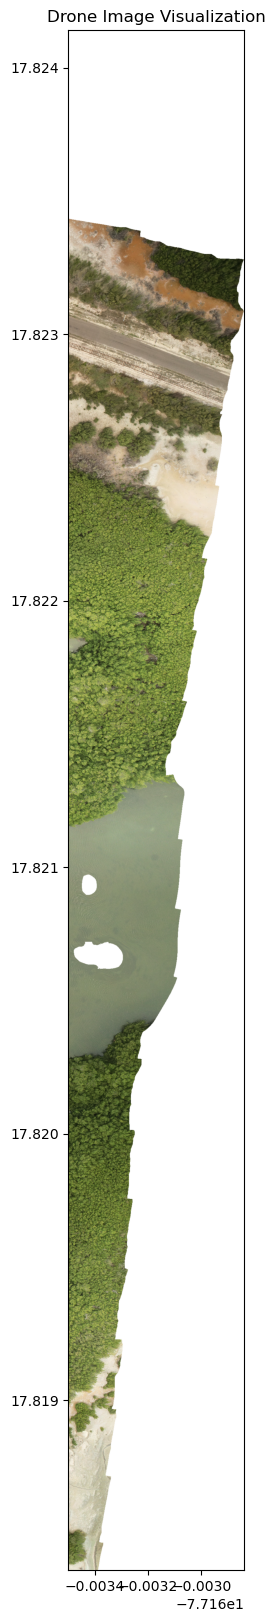
\includegraphics[width=0.4\textwidth, height=0.95\textheight]{images/Drone_tiff.png} \\
    \end{minipage}%
    \hfill
    \begin{minipage}[b]{0.49\textwidth}
        \centering
        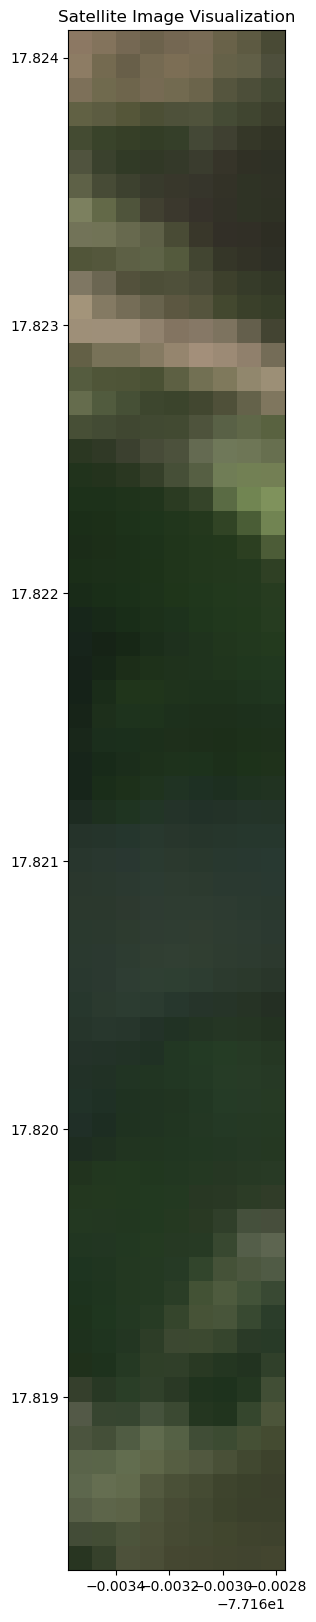
\includegraphics[width=0.4\textwidth,height=0.95\textheight]{images/Sat_tiff.png} \\
    \end{minipage}
\end{frame}


\begin{frame}{Super Resolution Training}
    \centering
    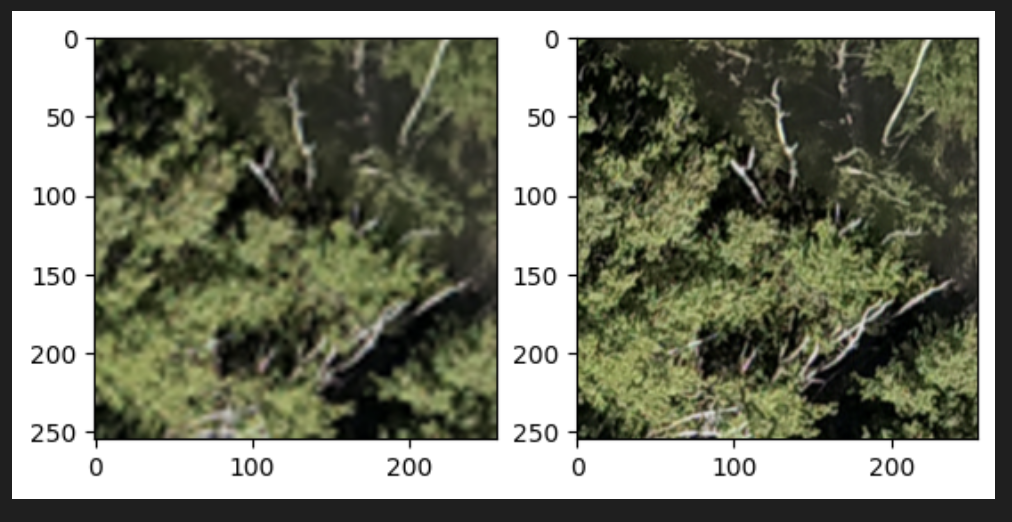
\includegraphics[height=0.5\textheight,width=0.6\textwidth,keepaspectratio]{images/Artificial_Downsample.png}
    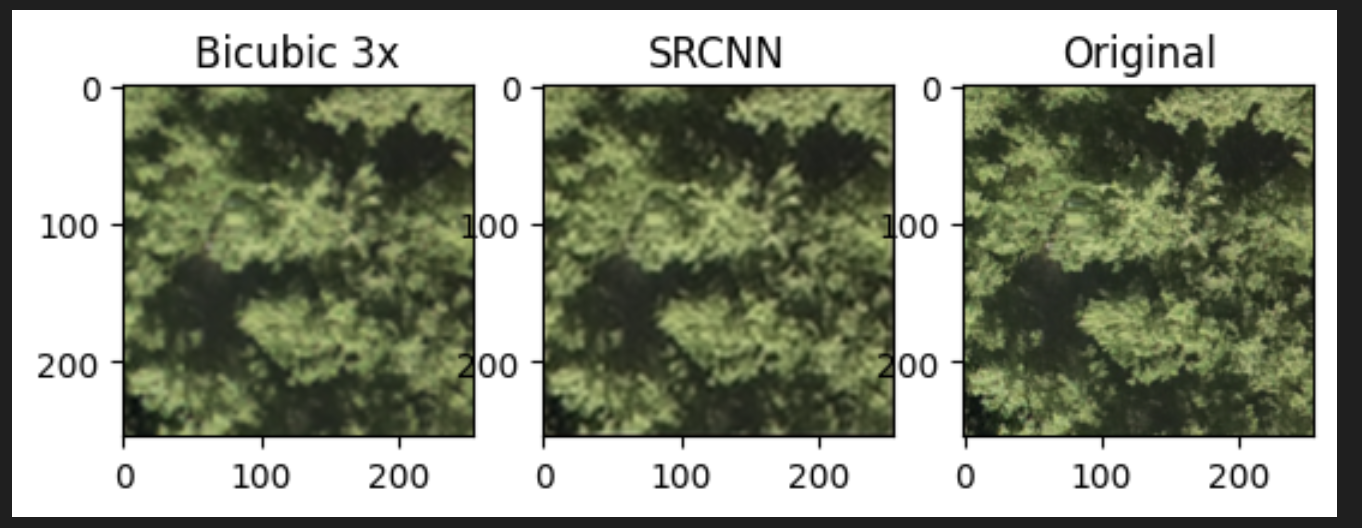
\includegraphics[height=0.5\textheight,width=0.6\textwidth,keepaspectratio]{images/Upsample_compare.png}
\end{frame}

\begin{frame}{Terraform Implementation}
    Divided across team AWS component-wise:
    \begin{itemize}
        \item EC2 Instance
        \item ECS Cluster
        \item ECR Repo
        \item S3 Bucket
        \item VPC (+ misc. odds and ends)
    \end{itemize}
\end{frame}

\begin{frame}{AWS Infrastructure Changes}
    \begin{itemize}
        \item Image preprocessing and classification moving to Kastner-ML
        \item TLS Authentication from Webserver to Kastner-ML
    \end{itemize}
\end{frame}

% To create a slide, use the following:
% \begin{frame}{TITLE}
%     BODY
% \end{frame}

% To create a slide with a bullet list, use the following:
% \begin{frame}{TITLE}
%     \begin{itemize}
%         \item ITEM 1
%         \item ITEM 2
%     \end{itemize}    
% \end{frame}

% To create a slide with numbered list, use the following:
% \begin{frame}{TITLE}
%     \begin{enumerate}
%         \item ITEM 1
%         \item ITEM 2
%     \end{enumerate}
% \end{frame}

% To create a slide with a graphic:
% 1. Add the graphic to this folder (named picture.png)
% 2. Use the following:
% \begin{frame}{TITLE}
%     \centering
%     \includegraphics[height=0.7\textheight,width=0.7\textwidth,keepaspectratio]{picture.png}
% \end{frame}

% To create a slide with two columns, use the following:
% \begin{frame}{TITLE}
%     \begin{columns}
%         \begin{column}{0.5\textwidth}
%             COLUMN 1 BODY
%         \end{column}
%         \begin{column}{0.5\textwidth}
%             COLUMN 2 BODY
%         \end{column}
%     \end{columns}
% \end{frame}
